% Dual-mode timing diagram: pull and push interaction over a 6-week task
\begin{figure}[t]
\centering
\resizebox{\textwidth}{!}{%
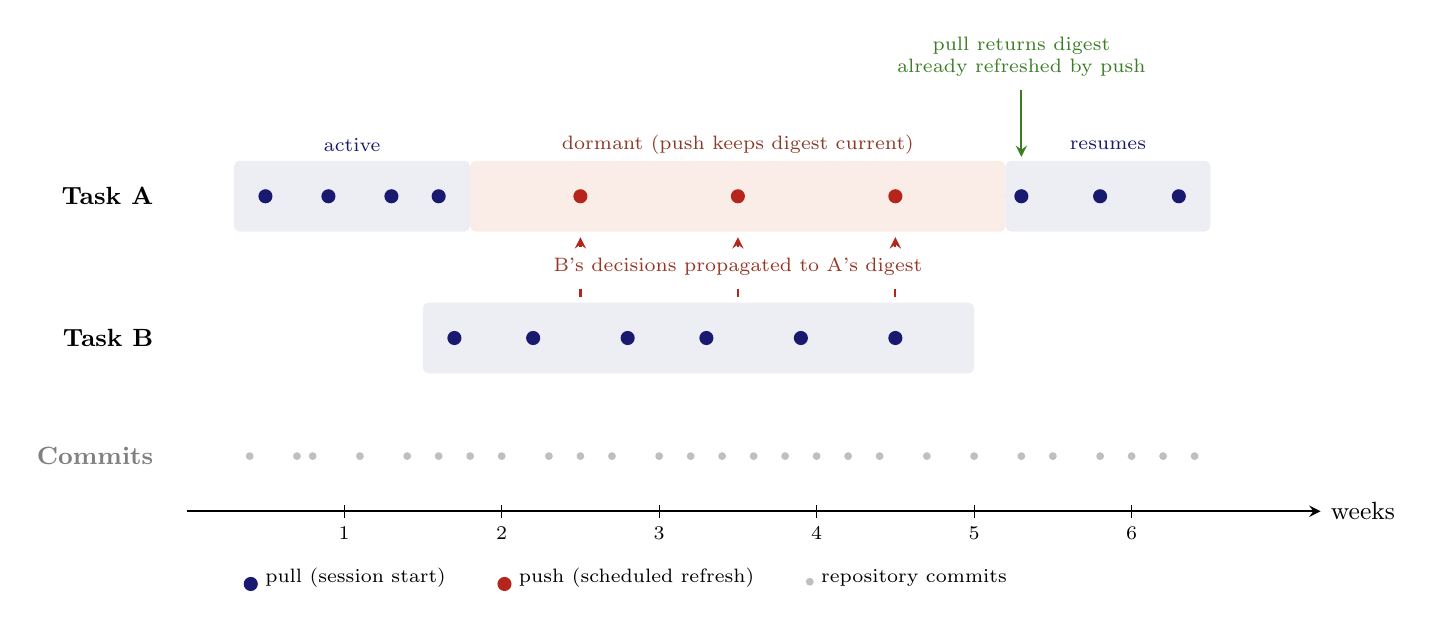
\begin{tikzpicture}[
    >=stealth,
    xscale=2.0,
    yscale=1.0,
    event/.style={circle, fill=#1, inner sep=1.8pt},
    pullev/.style={event=MidnightBlue},
    pushev/.style={event=BrickRed},
    commitdot/.style={event=gray!50, inner sep=1pt},
  ]

  % === Time axis ===
  \draw[->, thick] (0,-1.0) -- (7.2,-1.0) node[right, font=\small] {weeks};
  \foreach \w in {1,...,6} {
    \draw (\w, -0.92) -- (\w, -1.08) node[below, font=\scriptsize] {\w};
  }

  % === Task A timeline ===
  \node[font=\small\bfseries, anchor=east] at (-0.15, 3.0) {Task A};
  \draw[thick, gray!30] (0.3, 3.0) -- (6.5, 3.0);

  % Active/dormant shading
  \fill[MidnightBlue!8, rounded corners=2pt] (0.3, 2.55) rectangle (1.8, 3.45);
  \fill[BrickRed!6, rounded corners=2pt] (1.8, 2.55) rectangle (5.2, 3.45);
  \fill[MidnightBlue!8, rounded corners=2pt] (5.2, 2.55) rectangle (6.5, 3.45);

  % Phase labels above
  \node[font=\scriptsize, text=MidnightBlue] at (1.05, 3.65) {active};
  \node[font=\scriptsize, text=BrickRed!70!black] at (3.5, 3.65) {dormant (push keeps digest current)};
  \node[font=\scriptsize, text=MidnightBlue] at (5.85, 3.65) {resumes};

  % Pull events (blue dots)
  \foreach \x in {0.5, 0.9, 1.3, 1.6} { \node[pullev] at (\x, 3.0) {}; }
  \foreach \x in {5.3, 5.8, 6.3} { \node[pullev] at (\x, 3.0) {}; }

  % Push events (red dots, during dormancy)
  \foreach \x in {2.5, 3.5, 4.5} { \node[pushev] at (\x, 3.0) {}; }

  % === Task B timeline ===
  \node[font=\small\bfseries, anchor=east] at (-0.15, 1.2) {Task B};
  \draw[thick, gray!30] (1.5, 1.2) -- (5.0, 1.2);

  \fill[MidnightBlue!8, rounded corners=2pt] (1.5, 0.75) rectangle (5.0, 1.65);

  % Pull events
  \foreach \x in {1.7, 2.2, 2.8, 3.3, 3.9, 4.5} { \node[pullev] at (\x, 1.2) {}; }

  % === Cross-task propagation arrows ===
  \draw[->, BrickRed, thick, dashed, shorten >=2pt, shorten <=2pt]
    (2.5, 1.65) -- (2.5, 2.55);
  \draw[->, BrickRed, thick, dashed, shorten >=2pt, shorten <=2pt]
    (3.5, 1.65) -- (3.5, 2.55);
  \draw[->, BrickRed, thick, dashed, shorten >=2pt, shorten <=2pt]
    (4.5, 1.65) -- (4.5, 2.55);

  % Propagation label (single, centered)
  \node[font=\scriptsize, text=BrickRed!80!black, align=center, fill=white, inner sep=1.5pt]
    at (3.5, 2.1) {B's decisions propagated to A's digest};

  % === Key moment callout ===
  \draw[->, thick, OliveGreen] (5.3, 4.35) -- (5.3, 3.5);
  \node[font=\scriptsize, text=OliveGreen, align=center, anchor=south]
    at (5.3, 4.4) {pull returns digest\\already refreshed by push};

  % === Commit activity (bottom) ===
  \node[font=\small\bfseries, anchor=east, text=gray] at (-0.15, -0.3) {Commits};
  \foreach \x in {0.4, 0.7, 0.8, 1.1, 1.4, 1.6, 1.8, 2.0, 2.3, 2.5, 2.7, 3.0,
                   3.2, 3.4, 3.6, 3.8, 4.0, 4.2, 4.4, 4.7, 5.0, 5.3, 5.5, 5.8,
                   6.0, 6.2, 6.4} {
    \node[commitdot] at (\x, -0.3) {};
  }

  % === Legend ===
  \node[anchor=north west, font=\scriptsize] at (0.3, -1.6) {%
    \tikz[baseline=-0.5ex]\node[pullev] {};~pull (session start) \qquad
    \tikz[baseline=-0.5ex]\node[pushev] {};~push (scheduled refresh) \qquad
    \tikz[baseline=-0.5ex]\node[commitdot] {};~repository commits%
  };

\end{tikzpicture}%
}% end resizebox
\caption{Dual-mode retrieval over a six-week horizon with two concurrent tasks.
  Task~A is active in weeks~1--2, then dormant while Task~B runs in weeks~2--5.
  During dormancy, push-mode refresh propagates decisions from Task~B into Task~A's
  memory digest at a frequency proportional to commit activity.
  When Task~A resumes in week~5, the pull query returns context that is already current ---
  no expensive re-derivation required.
  Without push mode, the week-5 pull would return a stale digest from week~2, missing
  three weeks of relevant architectural decisions.}
\label{fig:dual-mode}
\end{figure}
